\documentclass[notes,11pt, aspectratio=169]{beamer}

\usepackage{pgfpages}
% These slides also contain speaker notes. You can print just the slides,
% just the notes, or both, depending on the setting below. Comment out the want
% you want.
\setbeameroption{hide notes} % Only slide
%\setbeameroption{show only notes} % Only notes
%\setbeameroption{show notes on second screen=right} % Both

\usepackage{helvet}
\usepackage[default]{lato}
\usepackage{array}
\usepackage{tgbonum}

\usepackage{tikz}
\usepackage{verbatim}
\setbeamertemplate{note page}{\pagecolor{yellow!5}\insertnote}
\usetikzlibrary{positioning}
\usetikzlibrary{snakes}
\usetikzlibrary{calc}
\usetikzlibrary{arrows}
\usetikzlibrary{decorations.markings}
\usetikzlibrary{shapes.misc}
\usetikzlibrary{matrix,shapes,arrows,fit,tikzmark}
\usepackage{amsmath}
\usepackage{mathpazo}
\usepackage{hyperref}
\usepackage{lipsum}
\usepackage{multimedia}
\usepackage{graphicx}
\usepackage{multirow}
\usepackage{graphicx}
\usepackage{dcolumn}
\usepackage{bbm}
\newcolumntype{d}[0]{D{.}{.}{5}}

\usepackage{changepage}
\usepackage{appendixnumberbeamer}
\newcommand{\beginbackup}{
   \newcounter{framenumbervorappendix}
   \setcounter{framenumbervorappendix}{\value{framenumber}}
   \setbeamertemplate{footline}
   {
     \leavevmode%
     \hline
     box{%
       \begin{beamercolorbox}[wd=\paperwidth,ht=2.25ex,dp=1ex,right]{footlinecolor}%
%         \insertframenumber  \hspace*{2ex} 
       \end{beamercolorbox}}%
     \vskip0pt%
   }
 }
\newcommand{\backupend}{
   \addtocounter{framenumbervorappendix}{-\value{framenumber}}
   \addtocounter{framenumber}{\value{framenumbervorappendix}} 
}


\usepackage{graphicx}
\usepackage[space]{grffile}
\usepackage{booktabs}

% These are my colors -- there are many like them, but these ones are mine.
\definecolor{blue}{RGB}{0,114,178}
\definecolor{red}{RGB}{213,94,0}
\definecolor{yellow}{RGB}{240,228,66}
\definecolor{green}{RGB}{0,158,115}

\hypersetup{
  colorlinks=false,
  linkbordercolor = {white},
  linkcolor = {blue}
}


%% I use a beige off white for my background
\definecolor{MyBackground}{RGB}{255,253,218}

%% Uncomment this if you want to change the background color to something else
%\setbeamercolor{background canvas}{bg=MyBackground}

%% Change the bg color to adjust your transition slide background color!
\newenvironment{transitionframe}{
  \setbeamercolor{background canvas}{bg=yellow}
  \begin{frame}}{
    \end{frame}
}

\setbeamercolor{frametitle}{fg=blue}
\setbeamercolor{title}{fg=black}
\setbeamertemplate{footline}[frame number]
\setbeamertemplate{navigation symbols}{} 
\setbeamertemplate{itemize items}{-}
\setbeamercolor{itemize item}{fg=blue}
\setbeamercolor{itemize subitem}{fg=blue}
\setbeamercolor{enumerate item}{fg=blue}
\setbeamercolor{enumerate subitem}{fg=blue}
\setbeamercolor{button}{bg=MyBackground,fg=blue,}



% If you like road maps, rather than having clutter at the top, have a roadmap show up at the end of each section 
% (and after your introduction)
% Uncomment this is if you want the roadmap!
% \AtBeginSection[]
% {
%    \begin{frame}
%        \frametitle{Roadmap of Talk}
%        \tableofcontents[currentsection]
%    \end{frame}
% }
\setbeamercolor{section in toc}{fg=blue}
\setbeamercolor{subsection in toc}{fg=red}
\setbeamersize{text margin left=1em,text margin right=1em} 

\newenvironment{wideitemize}{\itemize\addtolength{\itemsep}{10pt}}{\enditemize}

\usepackage{environ}
\NewEnviron{videoframe}[1]{
  \begin{frame}
    \vspace{-8pt}
    \begin{columns}[onlytextwidth, T] % align columns
      \begin{column}{.70\textwidth}
        \begin{minipage}[t][\textheight][t]
          {\dimexpr\textwidth}
          \vspace{8pt}
          \hspace{4pt} {\Large \sc \textcolor{blue}{#1}}
          \vspace{8pt}
          
          \BODY
        \end{minipage}
      \end{column}%
      \hfill%
      \begin{column}{.38\textwidth}
        \colorbox{green!20}{\begin{minipage}[t][1.2\textheight][t]
            {\dimexpr\textwidth}
            Face goes here
          \end{minipage}}
      \end{column}%
    \end{columns}
  \end{frame}
}

\title[]{\textcolor{blue}{Introduction to Applied Empirical Methods}}
\author[PGP]{}
\institute[FRBNY]{\small{Paul Goldsmith-Pinkham}}
\date{\today}


\begin{document}

%%% TIKZ STUFF
\tikzset{   
        every picture/.style={remember picture,baseline},
        every node/.style={anchor=base,align=center,outer sep=1.5pt},
        every path/.style={thick},
        }
\newcommand\marktopleft[1]{%
    \tikz[overlay,remember picture] 
        \node (marker-#1-a) at (-.3em,.3em) {};%
}
\newcommand\markbottomright[2]{%
    \tikz[overlay,remember picture] 
        \node (marker-#1-b) at (0em,0em) {};%
}
\tikzstyle{every picture}+=[remember picture] 
\tikzstyle{mybox} =[draw=black, very thick, rectangle, inner sep=10pt, inner ysep=20pt]
\tikzstyle{fancytitle} =[draw=black,fill=red, text=white]
%%%% END TIKZ STUFF

% Title Slide
\begin{frame}
\maketitle

\end{frame}

% INTRO
\begin{frame}{Assumed Background}
\begin{columns}[T] % align columns
\begin{column}{.7\textwidth}
  \begin{wideitemize}
  \item This class is targeted towards researchers interested in empirical work
  \item The course assumes exposure to Ph.D.-level econometrics material already
    \begin{itemize}
    \item E.g. first year sequence here at Yale
    \end{itemize}
  \item This is not because the material is deeply technical, but
    because I want to be able to assume some basic fluency in
    statistical concepts
  \end{wideitemize}
\end{column}%
\hfill%
\begin{column}{.38\textwidth}
  \makebox[\linewidth][c]{
    \resizebox{\linewidth}{!}{
%      \includegraphics{how-to-draw-an-owl.pdf}
    }
  }
\end{column}%
\end{columns}
\end{frame}

% INTRO
\begin{frame}{Requirements }
\begin{columns}[T] % align columns
\begin{column}{.9\textwidth}
  \begin{wideitemize}
  \item There are no exams, I will be assigning problem sets on a (quasi) weekly basis.
  \item You can use any computer package you wish to use. Solutions will be handed out written in R. 
    \begin{itemize}
    \item See syllabus for details
    \end{itemize}
  \item There are no required readings, but the papers listed in the    syllabus are relevant to the material we will cover in class. I will post lecture notes before class on the material along with the class slides.
  \item I also highly recommend the following texts:
    \begin{itemize}
    \item Angrist and  Pischke, Mostly Harmless Econometrics
    \item Hansen, Econometrics
    \item Miller and Aronow, Foundations of Agnostic Statistics
    \item Cunningham, Causal Inference: The Mixtape, https://mixtape.scunning.com/
    \item Imbens and Rubin, Causal Inference for Statistics, Social, and Biomedical Sciences      
    \end{itemize}
  \end{wideitemize}
\end{column}%
\hfill%
\begin{column}{.38\textwidth}
  \makebox[\linewidth][c]{
    \resizebox{\linewidth}{!}{
%      \includegraphics{how-to-draw-an-owl.pdf}
    }
  }
\end{column}%
\end{columns}
\end{frame}


% INTRO
\begin{frame}{Important caveat}
\begin{columns}[T] % align columns
\begin{column}{.7\textwidth}
  \begin{wideitemize}
  \item In the end, this is a graduate course targetted at making you a good empirical researcher
  \item My goal is to exposed to a wide range of empirical methods,
    and understand how they connect.
    \begin{itemize}
    \item We will not drill down deeply into some material
    \item I am happy to discuss it more outside of class
    \end{itemize}
  \item I will also emphasize how to communicate the econometrics underlying your research ideas
    \begin{itemize}
    \item This includes good graphic design!
    \end{itemize}
  \end{wideitemize}
\end{column}%
\hfill%
\begin{column}{.38\textwidth}
  \makebox[\linewidth][c]{
    \resizebox{\linewidth}{!}{
%      \includegraphics{how-to-draw-an-owl.pdf}
    }
  }
\end{column}%
\end{columns}
\end{frame}


\begin{frame}{Structure of the course}
  \begin{wideitemize}
  \item Six parts, first three are ``structure'' (12 lectures), second
    three parts are on different ``bespoke'' methods (12 lectures)
  \item We will begin with an overview on the structure for causal inference
  \item N.B. I am keeping everything on the github repo and will
    update you via Canvas notifications!
  \end{wideitemize}
\end{frame}


\begin{frame}{Introductions!}
    \resizebox{\linewidth}{!}{
      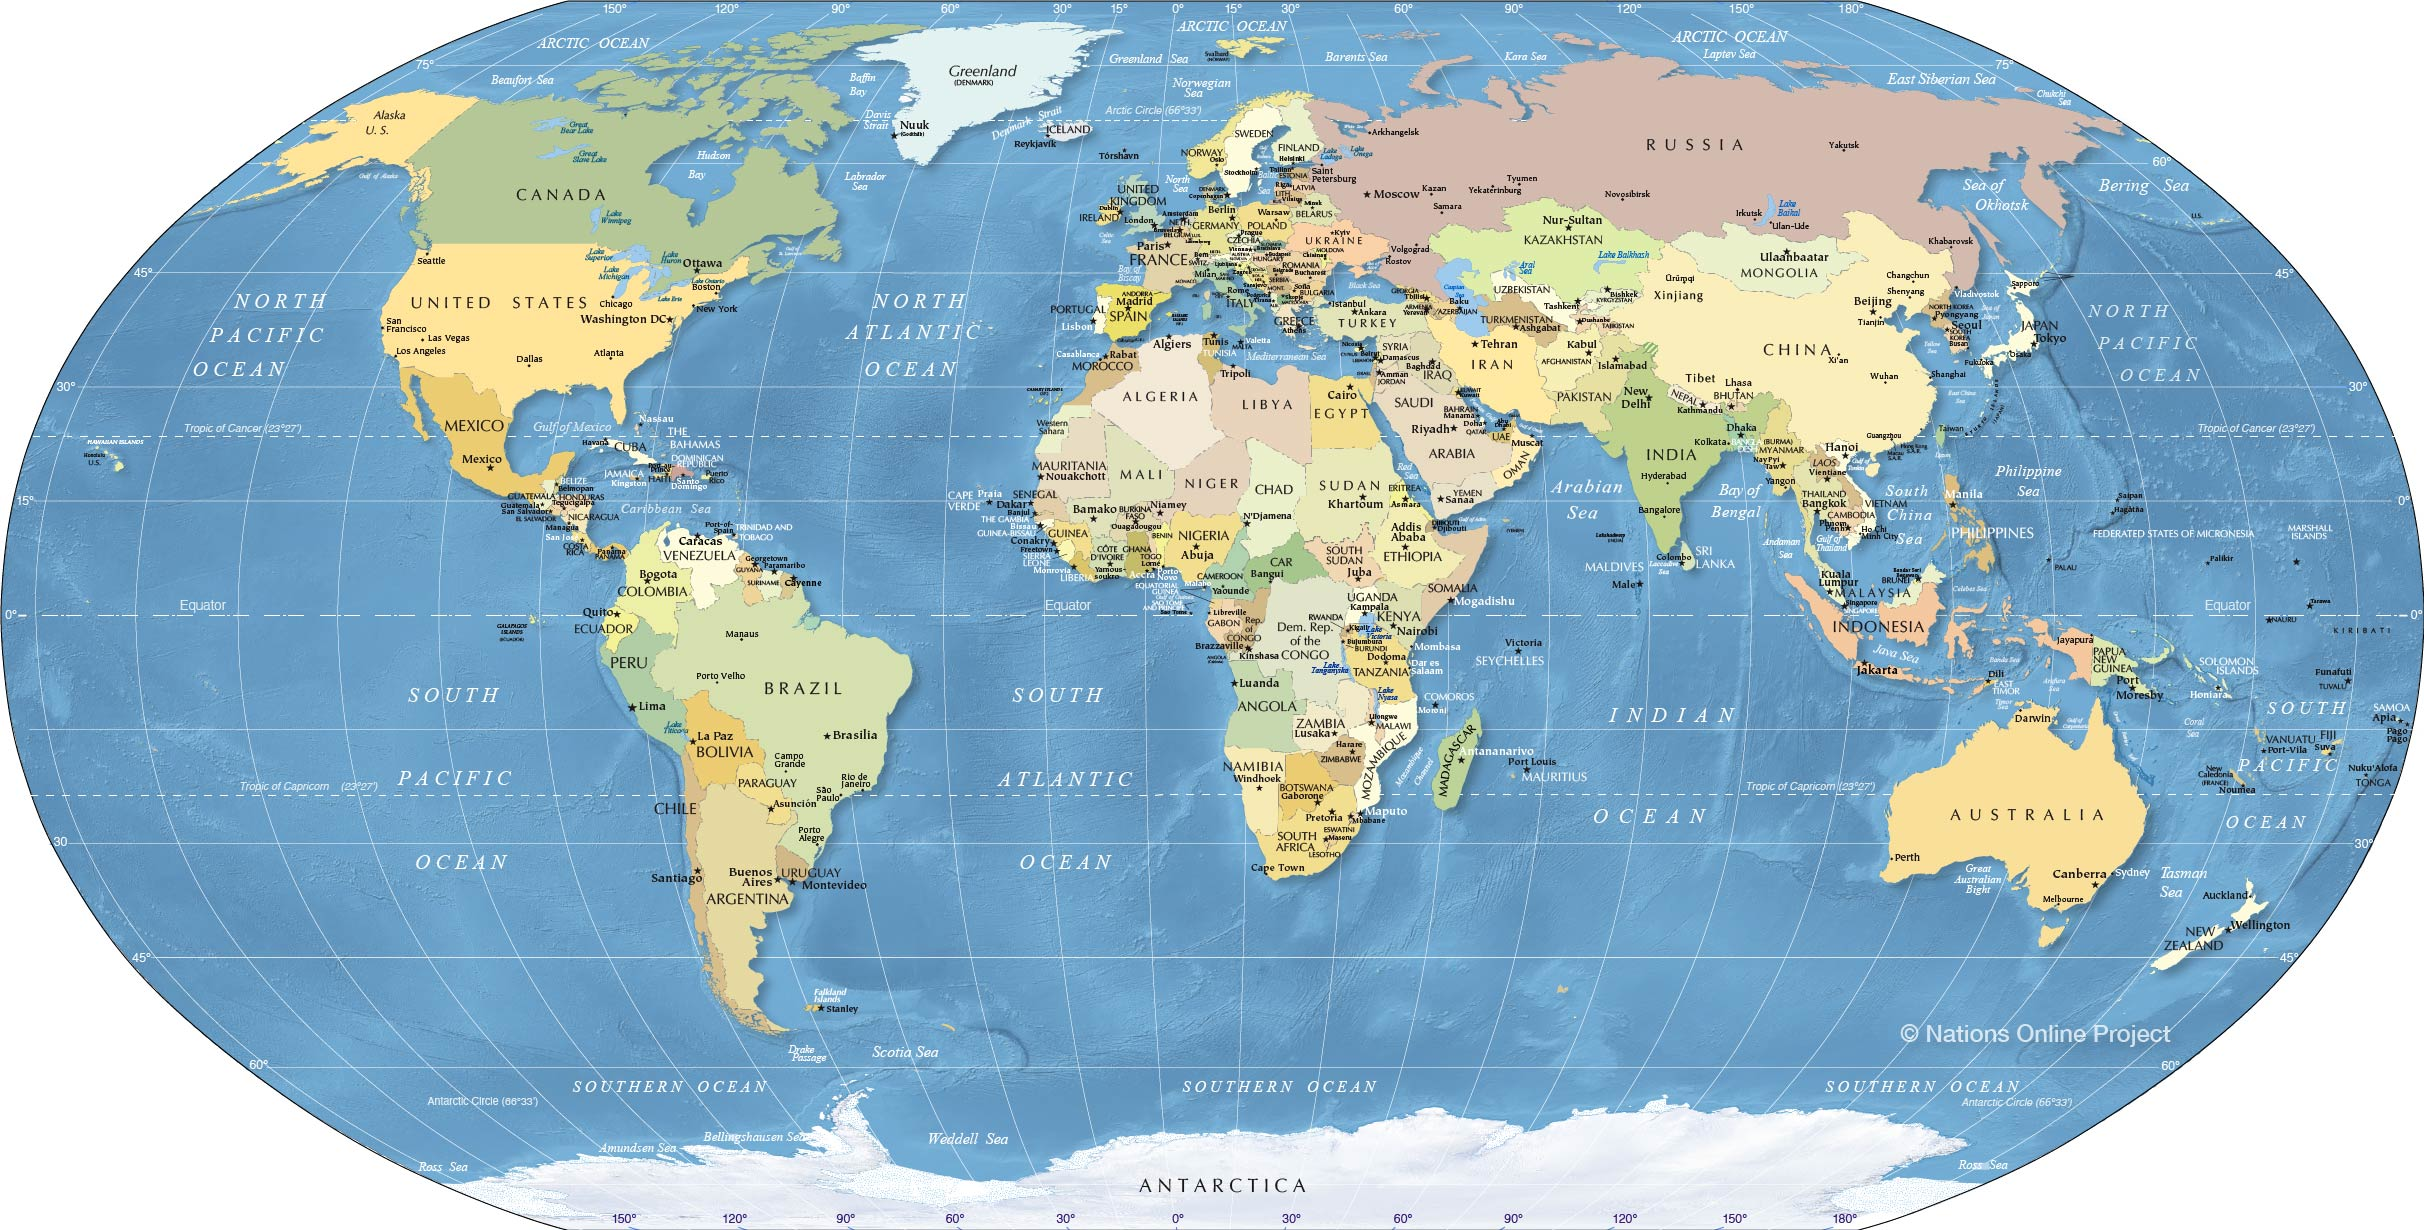
\includegraphics{images/map.jpeg}
    }
\end{frame}

\end{document}